\subsection{PSoC Master Implementering} \label{ch:master_psoc_impl}

På Figur \ref{fig:psoc_master_topdesign} ses topdesignet for PSoC Master projektet. 
Det ses hvordan der i det færdige design er udnyttet interrupts fra både UART og Timer. 
Disse har til formål at fortælle systemet når det er tid til hhv. at hente data fra UART og opdatere data fra sensorer.

\begin{figure}[h]
\centering
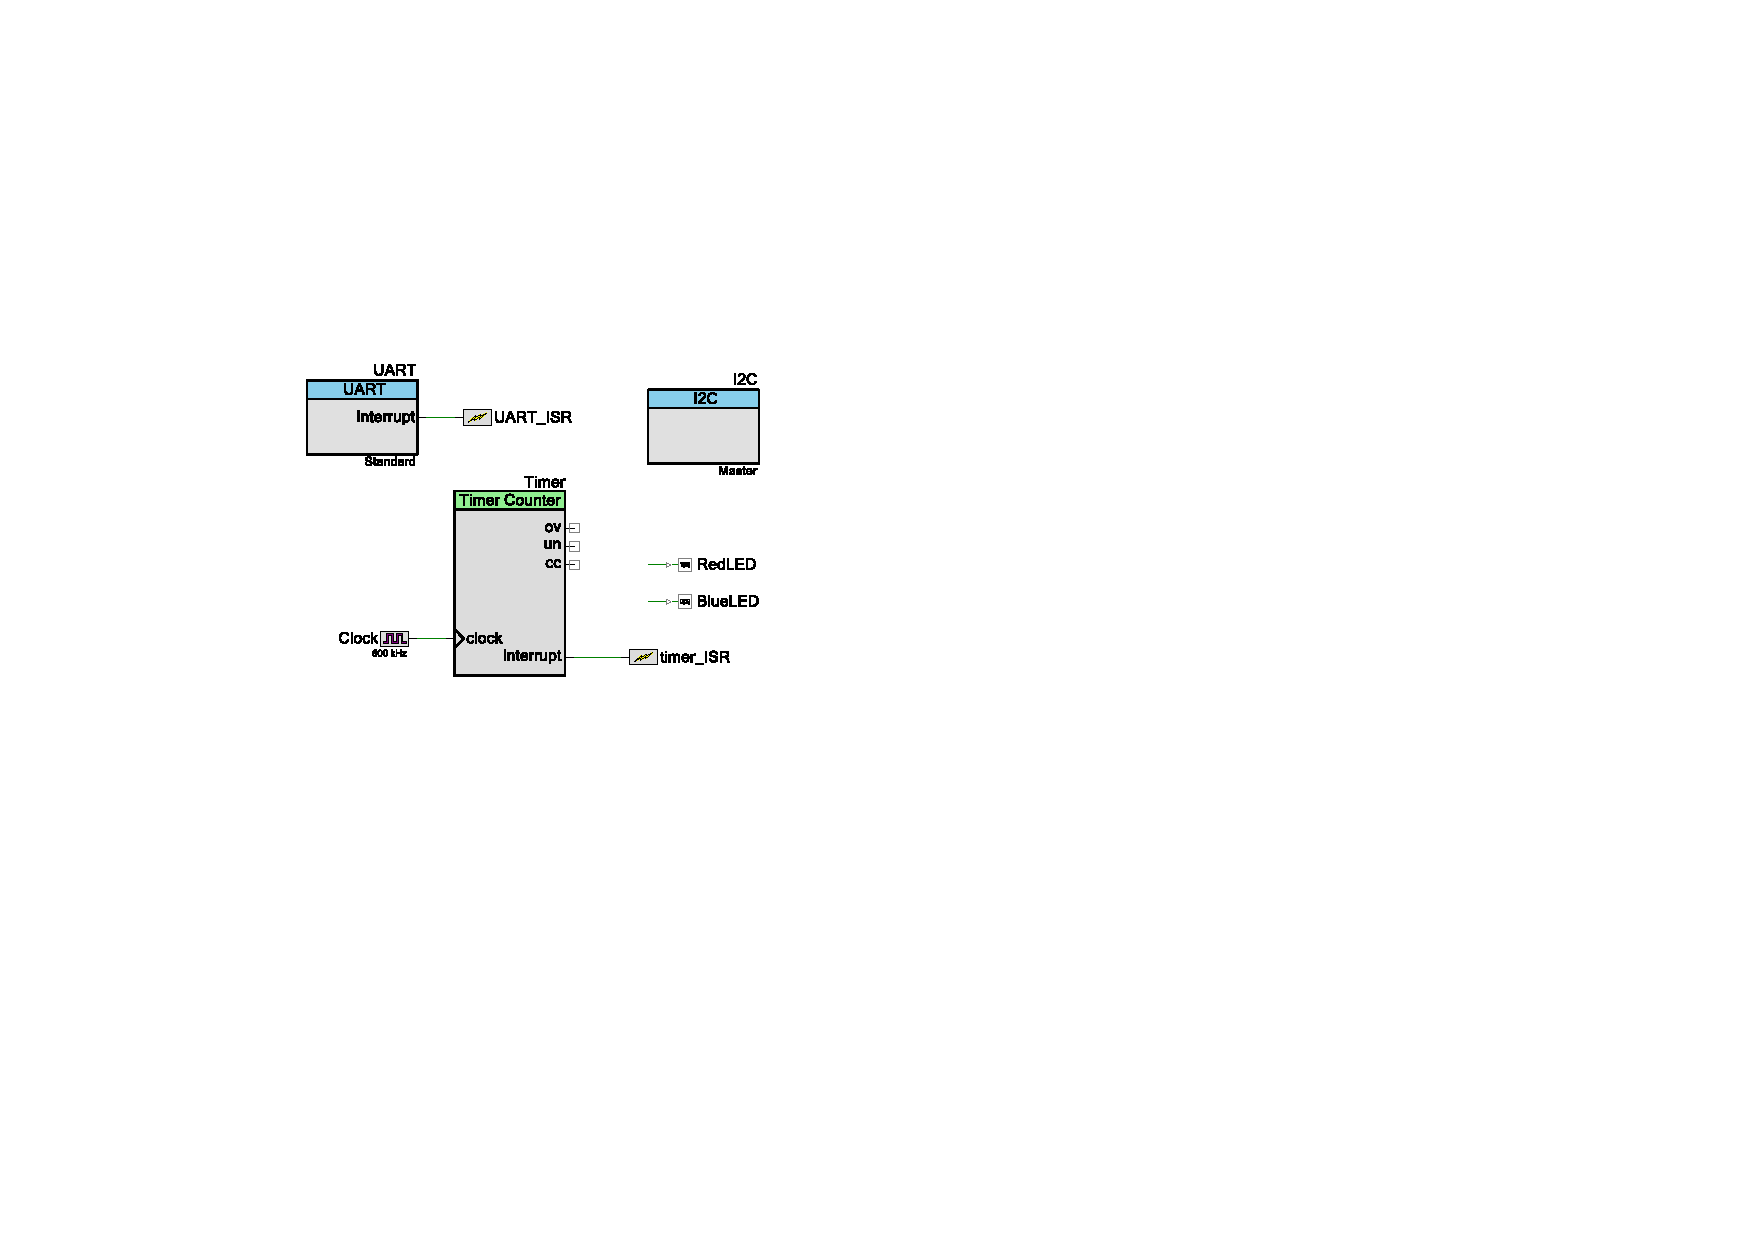
\includegraphics[width=\textwidth*7/10, trim=100 389 480 100, clip=true]{../fig/TopDesign_PSoC_Master}
\caption{Top Design for PSoC Master}
\label{fig:psoc_master_topdesign}
\end{figure}


%----------------------------Sensorer------------------------
Som udgangspunkt var der valgt en temperatur- og luftfugtighedssensor med navnet \textit{HONEYWELL S\&C  HIH6030-021-001} \cite{lib:TempHum_DS}. 
Arbejdet med denne sensor har ikke været problemfrit, da værdierne der kunne læses fra sensoren ikke var valide. 
Det var tydeligt at sensoren ikke afgav de korrekte værdier, da de lå fast på to forskellige størrelser, der i hvert fald ikke afspejlede virkeligheden. 
Om dette evt. skyldes en kortslutning eller at sensoren var brændt af, vides ikke.

Der blev valgt en ny temperatursensor (LM75\cite{lib:LM75}) som erstatning. Denne er dog uden mulighed for at måle luftfugtighed, men dette er acceptabelt, da det kun er temperaturen der er vigtig for systemets virkning. 
Lyssensoren \cite{lib:LightSens}, blev ligeledes nedprioriteret grundet tidsmangel og er derfor ikke implementeret.

\mbox{}

%-------------------------UART-----------------------
Gruppen har under udvikling af UART-delen til PSoC Master draget stor nytte af at UART kan kobles direkte på en PC. 
PSoC 4 Pioneer Kit giver via den monterede hjælpe-chip (PSoC 5) mulighed for at køre UART direkte fra USB og ud på PSoC 5'ens header.
Der er ligeledes under implementering af det færdige system brugt UART fra en PC til at sikre sig, at de givne input var korrekte i forhold til et svar fra systemet.

Ved implementering af UART klassen og \IIC klassen er der taget udgangspunkt i de respektive protokoller, der er beskrevet i dokumentationen i hhv. afsnit \ref{P-sec:UART_protokol} \nameref{P-sec:UART_protokol} på side \pageref{P-sec:UART_protokol} og afsnit \ref{P-sec:I2C_protokol} \nameref{P-sec:I2C_protokol} på side \pageref{P-sec:I2C_protokol}.

\mbox{}

%-------------------------integrationstest-------------------------------
Ved integrationstest med resten af systemet blev det valgt at timeren laver interrupt hvert andet sekund, hvilket betyder at alle sensordata også opdateres hvert andet sekund. Dette viste sig at give færrest problemer i kommunikationen mellem DevKit8000 og PSoC Master'en. 
Der kan i enkelte tilfælde stadig opstå en situation hvor kommunikationen her brister, hvilket resulterer i en fejlmeddelelse på systemets interface. Dette rettes dog allerede næste gang DevKit8000 efterspørger sensorværdier.

DSP klassen er implementeret, så der er mulighed for at variere hvor mange datapunkter, der skal midles over og dermed hvor lang tidsforsinkelse, der er på fx temperaturændringer. Her er der valgt, at der skal tages gennemsnittet af to punkter, hvilket giver en kort tidsforsinkelse, og derved er det lettere at regulere temperaturen i drivhuset.

\clearpage